\chapter{Conclusioni}

In questa trattazione si è dettagliato il meccanismo sotteso ai modelli probabilistici di diffusione del rumore (DDPM), che
hanno rappresentato un'innovazione nel contesto della modellaziome generativa, rivaleggiando con le GAN (Dhariwal e Nichol, $2021$~\cite{dhariwal2021}) 
nella generazione di immagini.
Dalla discussione del capitolo precedente emerge che il punto di forza dei DDPM è insito nell'alto grado di flessibilità 
offerto dagli stessi: l'unico requisito è che l'input e l'output della U-Net (Appendice~\ref{appendix:unet}) abbiano la stessa dimensionalità.


L'articolo pionieristico di Ho et al.\ (2020,~\cite{ho2020}) 
ha gettato le basi teoretiche per lo sviluppo di tecnologie quali Stable Diffusion\footnote{\url{https://stability.ai/}}, 
Imagen\footnote{\url{https://imagen.research.google/}}, DALL-E $2$\footnote{\url{https://openai.com/dall-e-2}}, 
il cui funzionamento sottende l'impiego di varianti del modello di diffusione descritto in questa tesi.

Sebbene le suddette tecnologie abbiano rivoluzionato l'ambito della generazione di immagini mediante l'uso dell'intelligenza artificiale, 
esse sollevano anche importanti implicazioni etiche.

Un primo problema risiede nel fatto che i modelli generativi di cui si avvalgono tali tecnologie riflettono 
i pregiudizi (\emph{bias}) impliciti nelle immagini del dataset di addestramento. Eloquente, a tal proposito, è la notizia, risalente al settembre $2022$, 
in cui si riporta che “\emph{OpenAI ha confermato a The Verge che DALL-E inserisce silentemente frasi nei prompt degli utenti per 
mitigare l'impatto dei bias insiti nelle immagini del dataset; ad esempio, le frasi «uomo di colore» e «donna asiatica» 
vengono inserite nei prompt che non specificano sesso o razza}”~\cite{DALLE2023}.

Infine, un'altra questione, molto delicata sotto il profilo etico, è il potenziale uso improprio di immagini generate dalle suddette tecnologie. 
In Figura~\ref{fig:amnesty} è riportata l'immagine, successivamente rimossa, pubblicata da \emph{Amnesty International} sul social media X, 
delle proteste colombiane del $2021$, mentre nel servizio di immagini stock di \emph{Adobe} 
si possono reperire foto, generate ricorrendo all'IA, concernenti il conflitto israelo-palestinese (Figura~\ref{fig:adobe}).

Benché le immagini in Figura~\ref{fig:concl} siano corredate dall'informazione di essere state create avvalendosi dell'intelligenza artificiale,
qualora, ad esempio, venissero immesse nel circuito dei mezzi d'informazione, sprovviste di segnalazioni esplicite sulla loro natura 
(da un'attenta analisi della Figura~\ref{fig:amnesty} risaltano i \emph{colori invertiti della bandiera colombiana}),
potrebbero essere impiegate per plagiare, subdolamente, il segmento con meno attitudine allo spirito critico dell'opinione pubblica. 
Ma questa è un'altra storia.
\begin{figure}
    \centering
    \subfloat[][Immagini pubblicate da \emph{Amnesty International}. Fonte:~\url{https://twitter.com}. \label{fig:amnesty}]
    {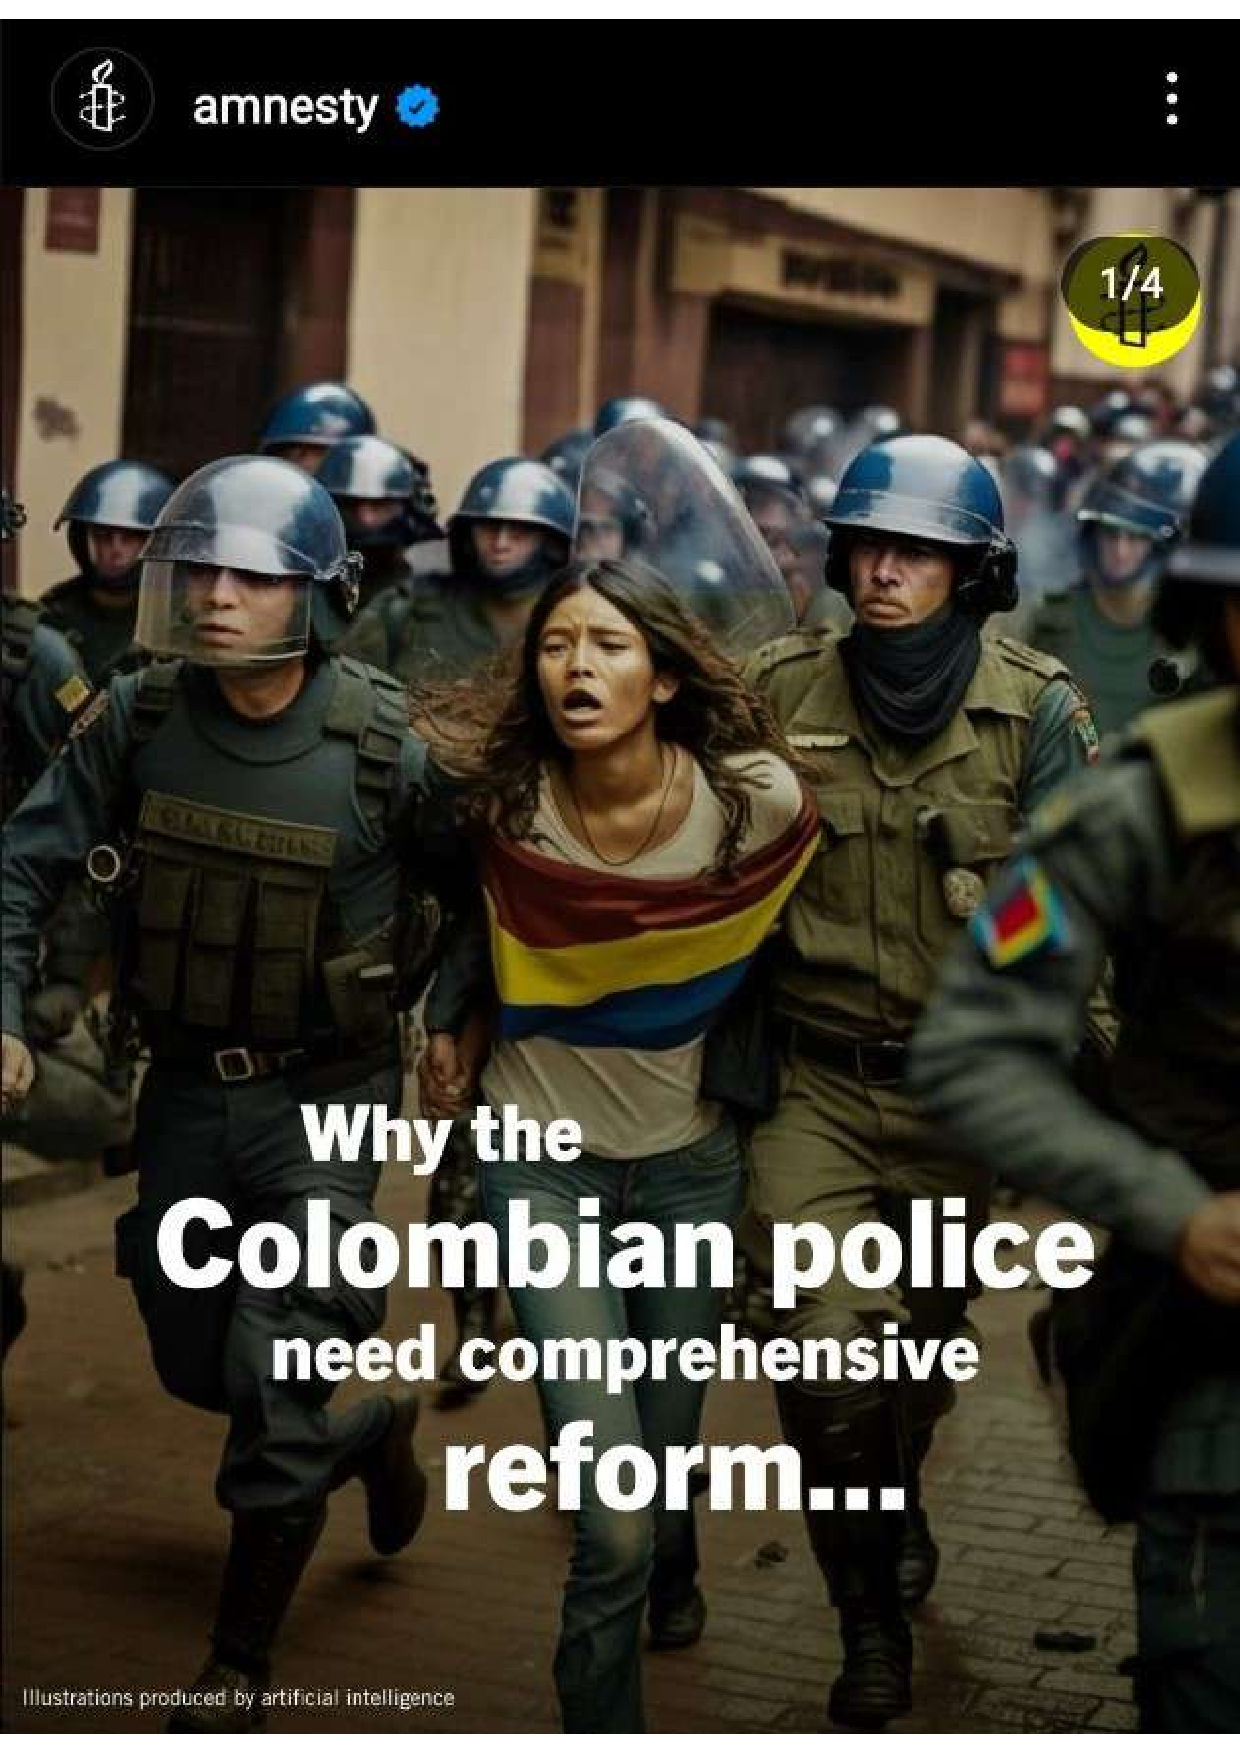
\includegraphics[keepaspectratio,scale=0.16]{amnesty_ai.pdf}} \quad
    \subfloat[][Immagini reperibili nel servizio immagini stock di \emph{Adobe}. Fonte:~\cite{wilsonAdobeSellingFake2023}. \label{fig:adobe}]
    {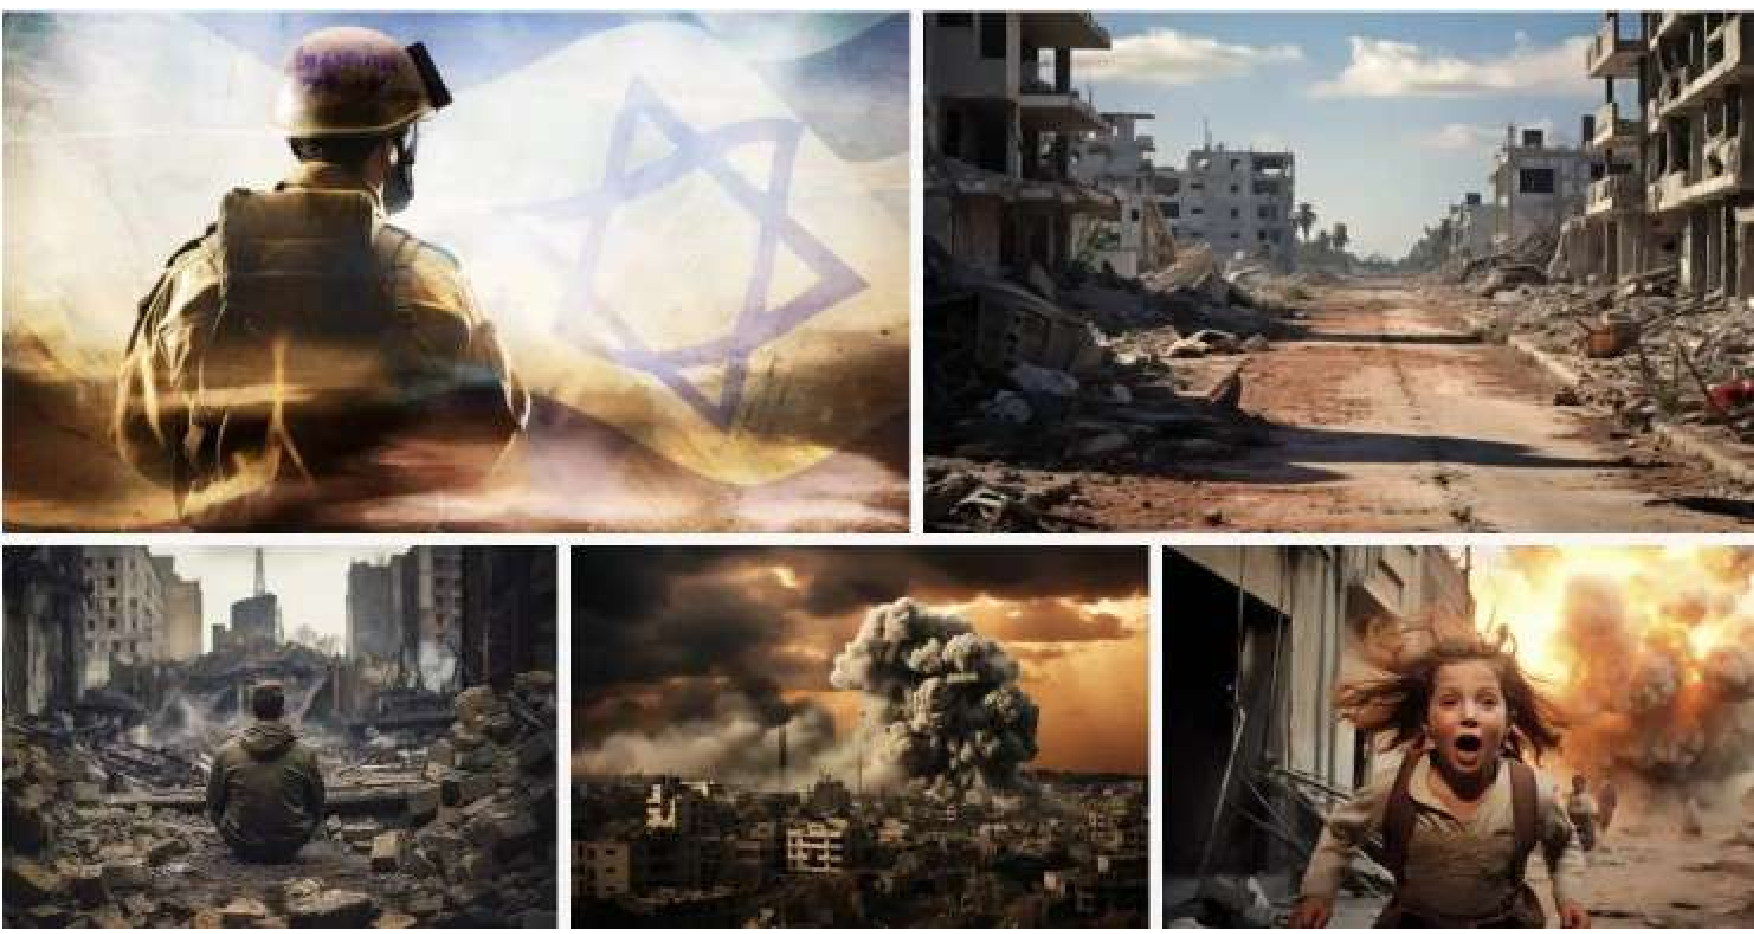
\includegraphics[keepaspectratio, scale=0.3]{adobe_ai.pdf}}
    \caption{Immagini create dall'intelligenza artificiale.}
    \label{fig:concl}
\end{figure}